\textbf{Работа 3.2.4}

\textbf{Свободные колебания в электрическом контуре}

\emph{Цель работы: исследование свободных колебаний в колебательном
контуре}

\emph{В работе используются: генератор импульсов, электронное реле,
магазин сопротивлений, магазин ёмкостей, катушка индуктивности,
электронный осциллограф, универсальный мост.}

Исследуемый колебательный контур состоит из индуктивности L, ёмкости C и
резистора R (рис. 2.1). Конденсатор контура заряжается короткими
одиночными импульсами, после каждого из которых в контуре возникают
свободные затухающие колебания. Подав напряжение с конденсатора на
осциллограф, можно по изображению на экране осциллографа определить
период свободных колебаний в контуре, исследовать их затухание и
определить основные параметры колебательного контура.

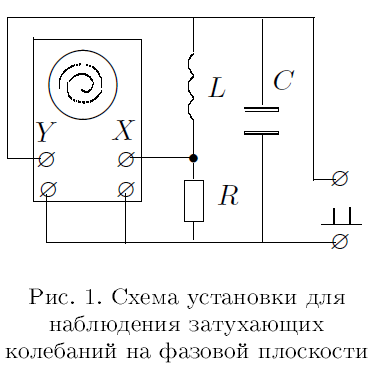
\includegraphics[width=2.275in,height=2.20833in]{./media/image1.png}Картину
колебаний можно представить не только в координатах (U,t) (рис. 2.2а),
но и в координатах (U, U̇) -- на так называемой \emph{фазовой плоскости}
(рис.2.2б). В этих координатах кривая незатухающих колебаний (при γ = 0)
имеет вид эллипса, а картина реальных затухающих колебаний представляет
собой сворачивающуюся спираль.

Принципиальная схема подключения осциллографа для изучения колебаний на
фазовой плоскости изображена на рис.1. На вертикальный вход осциллографа
подаётся напряжение Uc с конденсатора, а на горизонтальный -- напряжение
с резистора Ur (Ur \textasciitilde{} I \textasciitilde{}dq/dt
\textasciitilde{} dUc/dt).

\emph{\textbf{Экспериментальная установка.}} На рис.2 приведена схема
для исследования свободных колебаний в контуре, содержащем постоянную
индуктивность L и переменные ёмкость C и сопротивление R. Картина
колебаний наблюдается на экране осциллографа.

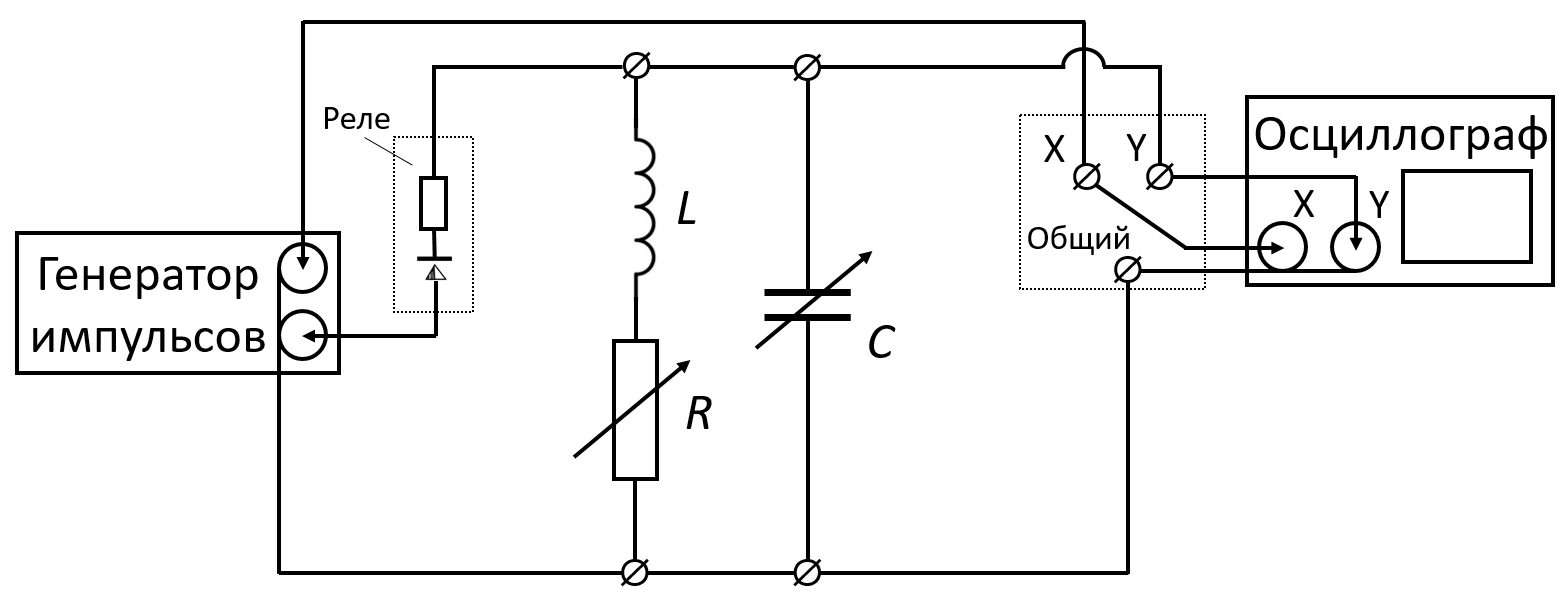
\includegraphics[width=6.49653in,height=2.48611in]{./media/image2.png}

Рис. 2. Схема установки для исследования свободных колебаний

Для периодического возбуждения колебаний в контуре используется
генератор импульсов. С выхода генератора сигналы поступают на
колебательный контур через электронное реле, которое содержит диодный
тиристор D и ограничительный резистор R1. Тиристор без управляющего
электрода представляет собой полупроводниковый ключ, открывающийся при
напряжении на нём выше порогового, и закрывающийся при любом напряжении
другого знака. Благодаря этому генератор отключается от колебательного
контура после каждого импульса, и внутреннее сопротивление генератора не
влияет на процессы в колебательном контуре.

Каждый импульс заряжает конденсатор C, после чего в контуре возникают
свободные затухающие колебания. Входное сопротивление осциллографа
велико, поэтому его влиянием на контур можно пренебречь.

\emph{\textbf{Задание}}

В работе предлагается исследовать зависимость периода свободных
колебаний контура от ёмкости, зависимость логарифмического декремента
затухания от сопротивления, определить критическое сопротивление и
добротность контура.

I. Подготовка приборов к работе

1. Соберите схему согласно рис.2. Подключите выход генератора через реле
к магазину ёмкостей таким образом, чтобы можно было менять ёмкость в
интервале 0 -- 1 мкФ.

2. Установите на генераторе длительность импульсов 5 мкс, а частоту
повторения импульсов ν0 = 100 Гц (T = 0,01~c).

3. Настройте осциллограф, руководствуясь техническим описанием,
расположенным на установке.

II. Измерение периодов свободных колебаний

4. Установите на магазине сопротивлений величину R = 0; на магазине
ёмкостей -- величину C = 0,02 мкФ.

5. Подберите частоту развёртки осциллографа, при которой расстояние
между импульсами, поступающими с генератора, занимает почти весь экран.

6. Измерьте расстояние, которое занимают несколько полных периодов n.
Проверьте, совпадают ли период повторения импульсов на генераторе с
периодом повторения импульсов, измеренным при помощи горизонтальной
шкалы осциллографа. При несовпадении периодов прокалибруйте
горизонтальную шкалу осциллографа по известному периоду повторения
импульсов.

7. Измерьте на экране осциллографа расстояние x, которое занимают
несколько полных периодов n. Рассчитайте период свободных колебаний
контура. Малые расстояния x можно увеличить кнопкой растяжки развёртки.

8. Изменяя ёмкость от 0,02 мкФ до 0,9 мкФ, проведите измерения периодов
свободных колебаний (8 -- 10 значений).

III. Измерение критического сопротивления и декремента затухания.

9. Для данной в работе индуктивности рассчитайте ёмкость C, при которой
собственная частота колебаний контура ν0 = 1/(2π√(LC)) составляет 5 кГц.
Для выбранных значений L и C рассчитайте критическое сопротивление
контура Rкр = 2√(L/C). (2.38)

10. Установите на магазине ёмкость, близкую к рассчитанной. Увеличивая
сопротивление R от нуля до Rкр, наблюдайте картину затухающих колебаний
на экране осциллографа. Зафиксируйте сопротивление магазина, при котором
колебательный режим переходит в апериодический. Сравните значения
найденного экспериментально и рассчитанного значения Rкр.

11. Установите сопротивление R ≃ 0,1 Rкр (эксп.). Получите на экране
картину затухающих колебаний. Для расчёта логарифмического декремента
затухания Θ по формуле (2.27) измерьте амплитуды, разделенные целым
числом периодов n. Расчёт будет тем точнее, чем больше отличаются друг
от друга измеряемые амплитуды, а минимальная не должна быть меньше 5 --
6 мм.

12. Повторите измерения для 6 -- 8 значений R в интервале (0,1 -- 0,3)
Rкр.

IV. Свободные колебания на фазовой плоскости.

13. Для наблюдения затухающих колебаний на фазовой плоскости подайте на
вход «Х» осциллографа напряжение с магазина сопротивлений.

Переведите осциллограф в режим измерения «X-Y». Изменяя чувствительность
каналов, подберите масштаб спирали.

При том же значении ёмкости что и в п. 10, наблюдайте за изменением
спирали при увеличении сопротивления от 0,1 до 0,3·Rкр.

Для определения Θ измерьте радиусы витков спирали, разделённые целым
числом периодов n, для одного-двух значений R на каждом краю рабочего
диапазона.

14. Отсоедините катушку от цепи. С помощью измерителя LCR измерьте
омическое сопротивление RLи индуктивность L катушки на частотах 50 Гц, 1
кГц и 5 кГц. Подумайте, почему результат измерения омического
сопротивления катушки зависит от частоты.

V. Обработка результатов.

15. Рассчитайте экспериментальные значения периодов по результатам
измерений (ч. II) и теоретические по формуле ν0 = 1/(2π√(LC)) (2.7).
Постройте график Тэксп=f(Tтеор).

16. Рассчитайте значения Θ (п.12) и Rконт (сопротивление контура состоит
из сопротивления магазина R и омического сопротивления катушки RL).

Постройте график в координатах 1/Θ\textsuperscript{2} =
f{[}1/(R\textsuperscript{2}конт){]}. Определите критическое
сопротивление Rкр по наклону прямой. С помощью равенств (2.6), (2.23),
(2.27), и (2.38) и приняв обозначения 1/Θ2=Y, 1/Rконт2 = X, покажите,
что Rкр = 2π√(ΔY/ΔX).

17. Рассчитайте теоретическое значение Rкр = 2√(L/C) (2.38) и сравните
его с измеренным.

18. Рассчитайте добротность контура Q для максимального и минимального
значений Θ по картине затухающих колебаний и сравните с расчётом Q через
параметры контура R, L и С (см 2.34).

19. Рассчитайте добротность Q по спирали.

20. Сведите результаты эксперимента в таблицу:

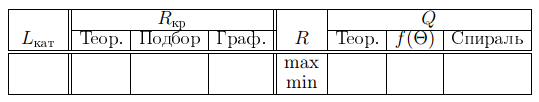
\includegraphics[width=4.85833in,height=0.91939in]{./media/image3.png}

21. Оцените погрешности и сравните результаты. Какой из методов
определения Rкр и Q точнее?

Контрольные вопросы.

\begin{enumerate}
\def\labelenumi{\arabic{enumi}.}
\item
  Что такое собственная частота, добротность, логарифмический декремент
  затухания колебательного контура?
\item
  Что называют фазовой плоскостью колебаний?
\item
  Как определить логарифмический декремент затухания по картине
  колебаний в фазовой плоскости?
\item
  Возможно ли вызвать резонанс в колебательном контуре при помощи
  периодических импульсов?
\end{enumerate}

Список литературы.

1. \emph{Сивухин} Д.В. Общий курс физики. -- Т.III. Электричество. --
М.: Физматлит, 2004. §§ 122 -- 124.

2. \emph{Калашников С.Г.} Электричество. -- М.: Физматлит, 2008. §§ 207
-- 210.
